% !TeX spellcheck = en_US
% !TXS template
\documentclass[english]{article}
\usepackage[T1]{fontenc}
\usepackage[utf8]{inputenc}
\usepackage{lmodern}
\usepackage[a4paper]{geometry}
\usepackage{babel}
\usepackage{amsmath}
\usepackage{amsfonts}
\usepackage{amsthm}
\usepackage{amssymb}
\usepackage{mathtools}
\usepackage[backend=bibtex,style=alphabetic]{biblatex}
\usepackage{csquotes}
\usepackage{algorithm}
\usepackage{algpseudocode}
\usepackage{hyperref}
\usepackage[most]{tcolorbox}
\usepackage{enumitem}
\usepackage{fancyvrb}
\usepackage{multicol}
\usepackage{stmaryrd}
\usepackage{tikz}
\usepackage{graphicx}
\usepackage{caption}
\usepackage[affil-it]{authblk}

\usetikzlibrary{arrows.meta, positioning}

\addbibresource{biblio.bib}

\graphicspath{./}

\newlength{\participantimgsize}
\setlength{\participantimgsize}{1.8cm}

\newtheorem{proposition}{Proposition}[section]
\newtheorem{definition}{Definition}[section]
\newtheorem{theorem}{Theorem}[section]
\newtheorem{corollary}{Corollary}[section]
\newtheorem{lemma}{Lemma}[section]
\newtheorem{example}{Example}[section]

\newcommand{\Mac}[3]{{Mac_{#1, #2}(\mathcal{#3})}}
\newcommand{\Mact}[3]{{\widetilde{Mac}_{#1, #2}(\mathcal{#3})}}
\newcommand{\lir}{\llbracket i \rrbracket}

\newcommand{\propositionTitre}[2]{
	\begin{proposition}[#1]
		#2
	\end{proposition}
}

\author{Paul Mekhail
	\thanks{\texttt{paul.mekhail4@pm.me}}}
\affil{Laboratoire MIS, Université de Picardie Jules Verne, Amiens, France\\Sorbonne Université, Paris, France}

\author{\textbf{Advisor}: Sorina Ionica
	\thanks{\texttt{sorina.ionica@u-picardie.fr}}}
\affil{Laboratoire MIS, Université de Picardie Jules Verne, Amiens, France}

\title{Cryptanalysis of SBC based post-quantum signature scheme \\\textit{Graduation internship report}}

\begin{document}
	\maketitle
	
	\section{Introduction}
		Since the emergence of quantum computing in the late 1990s, several breakthroughs have been achieved in the field of quantum algorithms. Some of these advancements have found applications in areas such as medicine and physics, while others have demonstrated the ability to break cryptographic problems that are currently assumed to be hard for classical computers, such as RSA \cite{RSA78} and ECDH.
		
		In particular, quantum algorithms like Grover's \cite{Grover} and Shor's \cite{Shor} have shown that existing public-key cryptosystems are vulnerable in a post-quantum setting. This has led to an urgent need for new hard problems on which to base quantum-resistant public-key cryptography.
		
		Post-quantum cryptographic schemes are generally built upon four main problem classes: isogeny-based, multivariate, code-based, and lattice-based cryptography. In recent years, new paradigms have also been explored to improve the efficiency and security of schemes within these classes. One such paradigm is the \emph{MPC-in-the-Head} approach.
		
		Although these underlying problems are believed to be hard even for quantum computers, some have been shown to be vulnerable to classical attacks due to hidden structures. A notable example is the NIST finalist Rainbow \cite{JD05}, a multivariate signature scheme that was broken in 2022 by Beullens \cite{Beu22} through exploitation of structural weaknesses.
	
		
		One might argue that post-quantum cryptography is not yet necessary, given that large-scale quantum computers capable of breaking classical cryptography do not currently exist. However, adversaries could perform so-called \emph{harvest-and-decrypt-later} attacks, in which encrypted data is collected today and decrypted in the future when quantum capabilities become available.
		
		In response to these concerns, the National Institute of Standards and Technology (NIST) launched an international competition in 2016 to standardize post-quantum cryptographic primitives.
	
		The \emph{MPC-in-the-Head} (MPCitH) paradigm, first introduced in \cite{IKOS07}, has recently gained significant attention—particularly in the second round of NIST’s post-quantum signature standardization process, where 5 out of 14 candidate schemes were based on this approach.
		
		The core idea of this paradigm is to leverage an NP-relation $\mathcal{R}(x, w)$ to construct a zero-knowledge (ZK) protocol. In such a protocol, a prover $\mathcal{P}$ convinces a verifier $\mathcal{V}$ that they possess a valid witness $w$ for a given public input $x$, without revealing any additional information about $w$.
		
		The main appeal of the MPCitH paradigm lies in the fact that it enables the construction of efficient, non-interactive, and quantum-resistant signature schemes with relatively small signature sizes and low verification cost and extremely small keys size.
		
		In~\cite{HJ23}, the authors introduced the \emph{Subfield Bilinear Collision} (SBC) problem, which is rooted in the hardness of the discrete logarithm problem \cite{Joux13}. Based on this assumption, they proposed a post-quantum signature scheme constructed using the MPCitH framework.
		
		The objective of this internship is to conduct a cryptanalysis of this scheme, assess its security and efficiency, and explore potential improvements.
		This includes evaluating its concrete security parameters and identifying potential structural weaknesses.
		
		In Section~\ref{sec2}, we introduce the MPCitH paradigm and provide an overview of the SBC problem, including its variants as well as the identification and signature schemes built upon it. 
		
		In Section~\ref{sec3}, we present key results in polynomial system solving and describe the main algorithms and results used in our cryptanalysis.
		
		Finally, in Section~\ref{sec4}, we detail our contributions, including the cryptanalysis and formal security evaluation of the SBC-based signature scheme, and summarize the most efficient known attacks against it.
	
		\begin{figure}[H]
			\begin{center}
				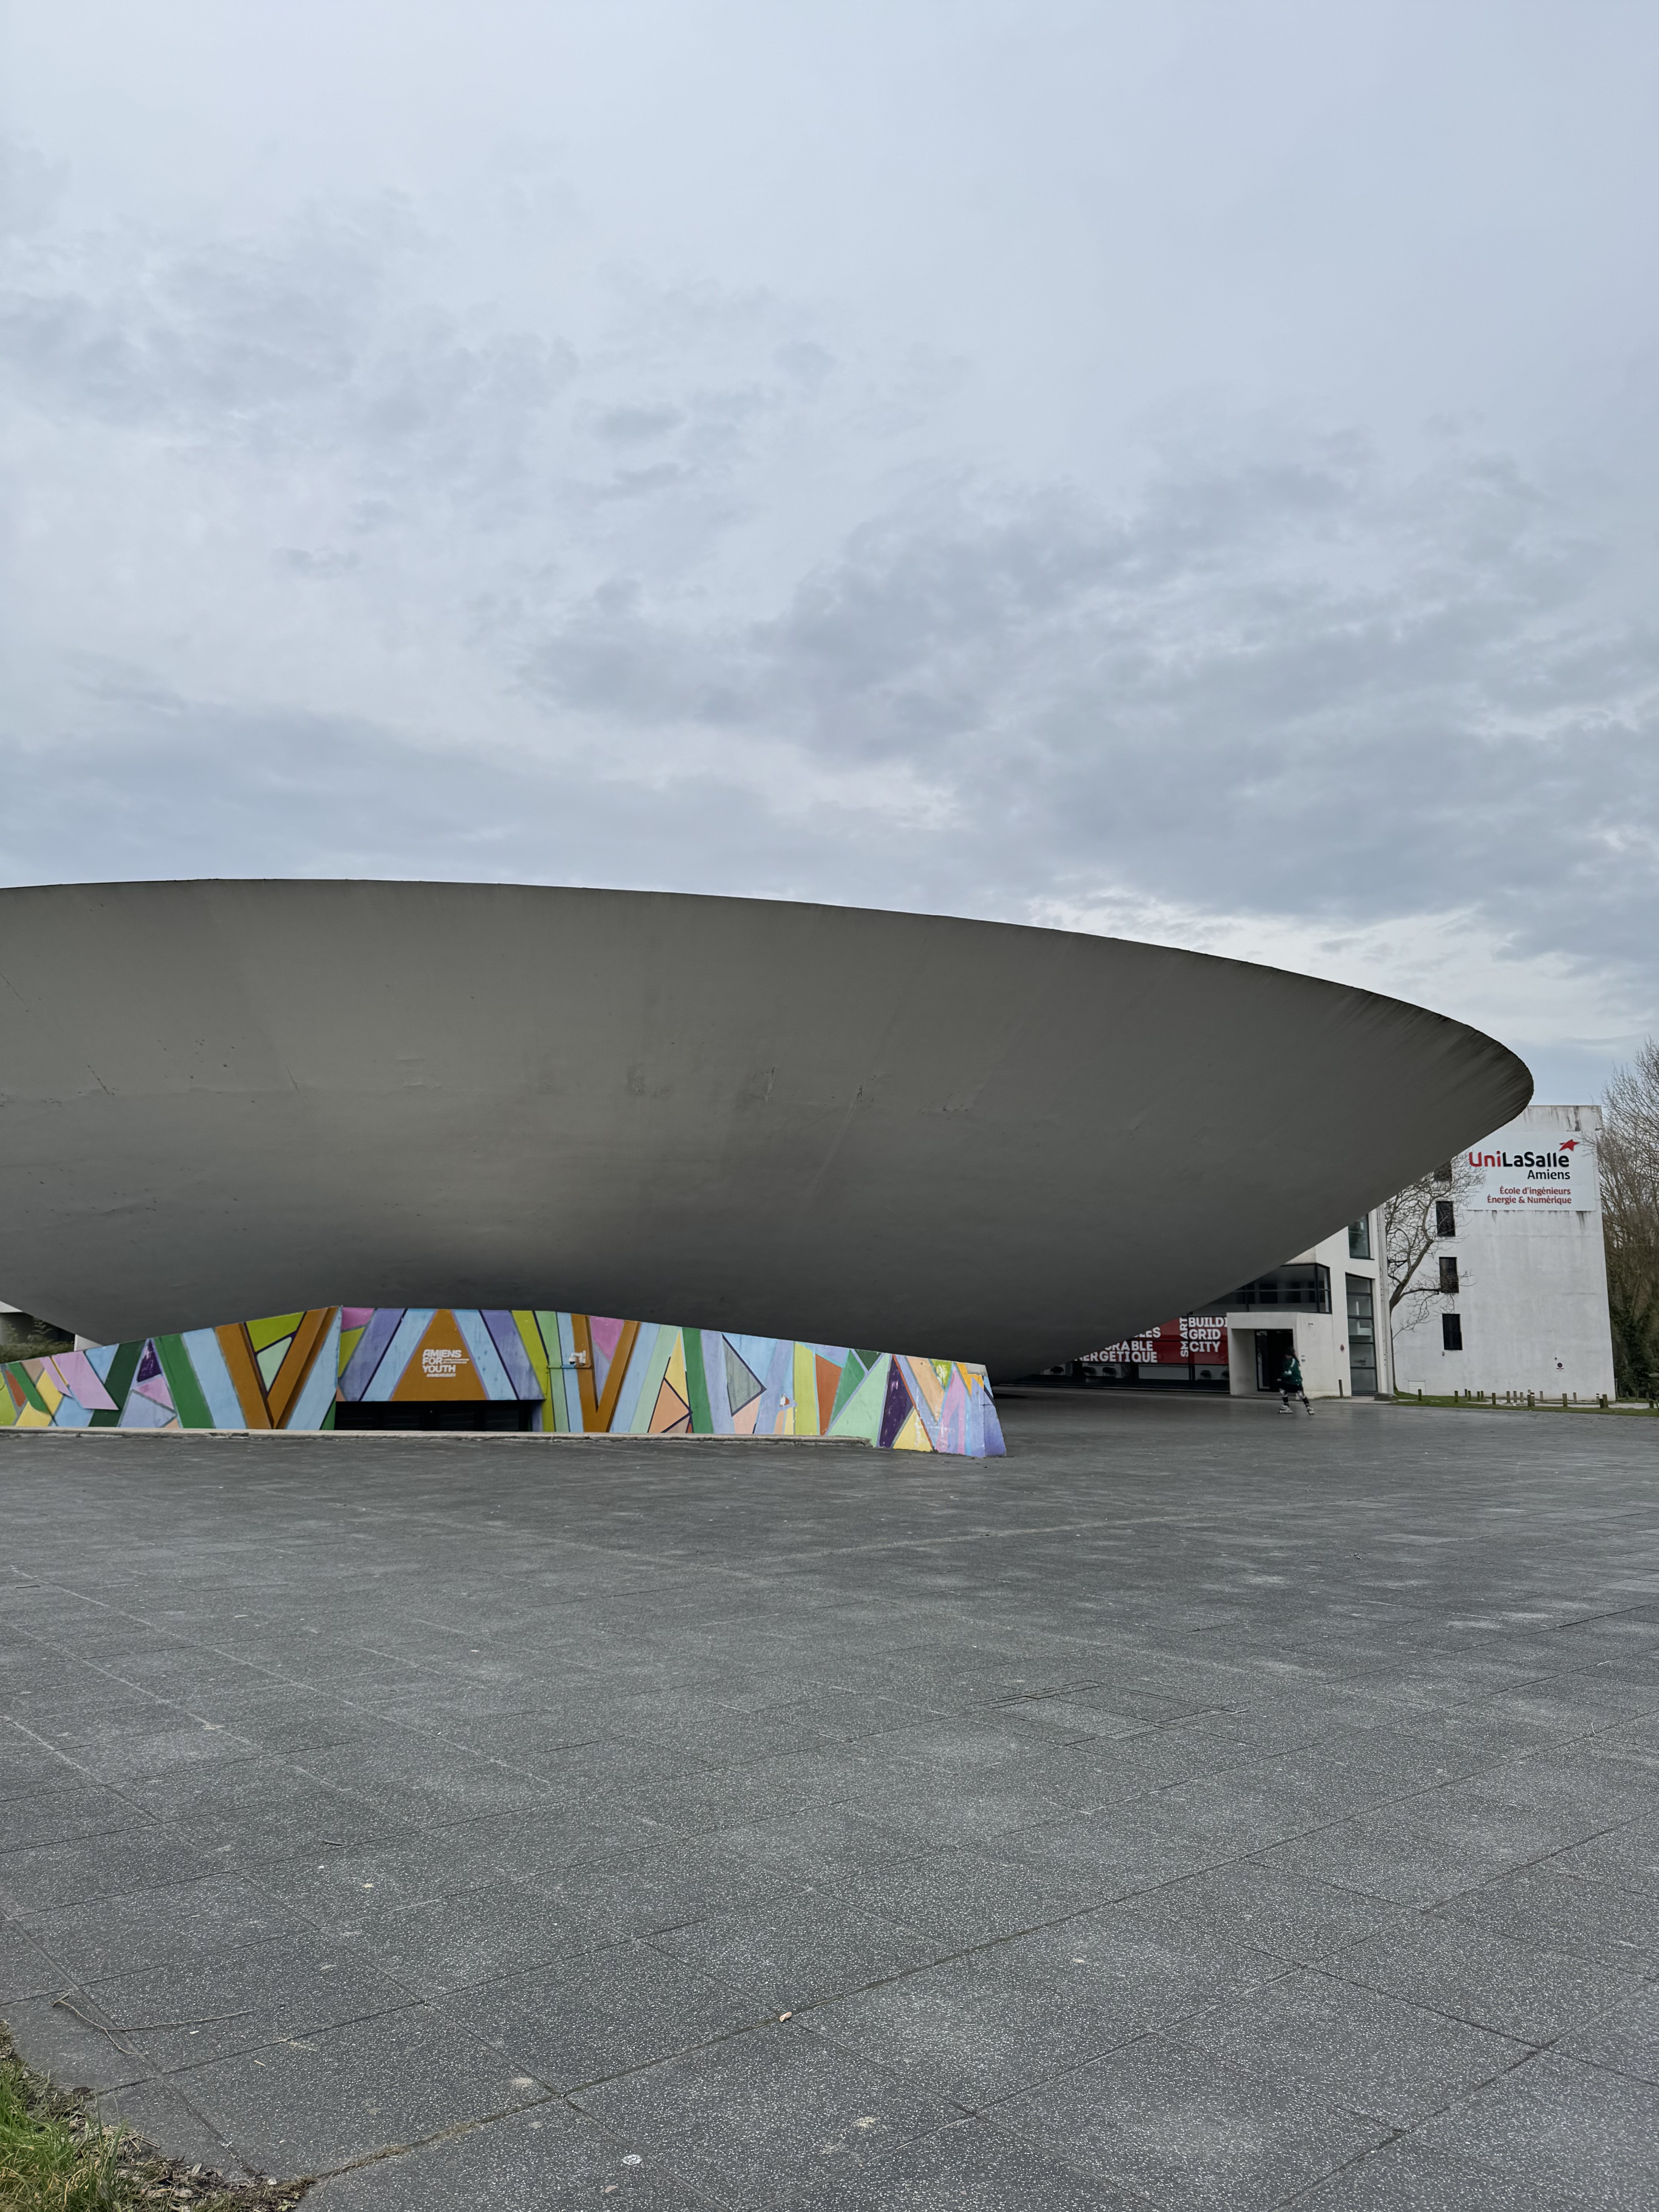
\includegraphics[scale=0.04]{unilasalle.jpg}
				\caption{UniLaSalle Engineering School, where the MIS offices are located(for now). Observant readers may notice the unusual UFO-like structure situated in front of the building.}
			\end{center}	
		\end{figure}
	
	\newpage
	\tableofcontents
	\newpage
	\section{MPCitH and SBC signature scheme}\label{sec2}
		
		\subsection{MPCitH}
		
		The \emph{MPC-in-the-Head} (MPCitH) framework, introduced by \cite{IKOS07}, is a technique for constructing zero-knowledge proofs. It enables a prover to convince a verifier that they possess a secret witness $w$ for a given public input $x$, without revealing any information about the witness itself.
		
		Given $\mathcal{L}$ a language in NP (i.e. $x \in \mathcal{L} \Longleftrightarrow \exists w, \mathcal{R}(x, w) = 1$). Given a public $x$, $\mathcal{P}$ wants to prove that he knows $w$ such that: $\mathcal{R}(x, w)$.
		
		The main idea is to simulate a secure multiparty computation (MPC) protocol internally \textit{in the head} of the prover $\mathcal{P}$. This simulation involves a set of fictitious parties who jointly evaluate a circuit that depends on the witness $w$. The verifier $\mathcal{V}$ is then allowed to inspect a subset of the simulated views to ensure the prover is behaving honestly, while maintaining the zero-knowledge property.
		
		To represent the secret witness $w$, a linear secret sharing scheme is used among $N$ simulated parties. Each party $i$ receives a random share denoted by $[w]^{\lir}$, and the prover computes an additional correction term defined as:
		$$
		\delta_w = w - \sum_{i=1}^{N} [w]^{\lir}.
		$$
		This ensures that the full witness can be correctly reconstructed from the shares and the correction term during the simulated execution.
		
		Next, the prover $\mathcal{P}$ commits to the views of the $N$ fictitious parties, denoted as $View_i$, and sends these commitments to the verifier $\mathcal{V}$. Each view contains all messages sent and received by the corresponding party during the simulated execution of the MPC protocol.
		
		The verifier $\mathcal{V}$ then selects a random index $i \in [1, N]$ and sends it to $\mathcal{P}$. In response, $\mathcal{P}$ opens the views of all parties except the $i$-th one, i.e., for all $i' \in [1, N]$ such that $i' \neq i$.
		
		In order for this protocol to satisfy the zero-knowledge property, the underlying MPC protocol must be $(N-1)$-private, meaning that the joint view of any $N-1$ parties reveals no information about the secret witness $w$.
		
		We introduce some standard notations in MPCitH protocols. 
		\begin{itemize}
			\item $[w]$, $w$ is a shared value.
			\item $w^{\lir}$ is the $i$-th share of w.
			\item $w^[e]$ is a value used in the $e$-th round of the protocol.
			\item $\delta_x$ is the offset for the additive sharing of $x$ s.t. $x = \delta_x + \sum_i x^{\lir}$
		\end{itemize}
		
		Finally, we discuss several optimizations that have been proposed in the literature since and are now considered standard and widely used.
		
		\subsubsection{GGM tree}
		Since most of the values used in the MPC protocol are randomly generated, a technique known as the GGM tree can be employed to transmit only a seed, rather than all the individual random values. This technique has been introduced in \cite{GGM86}.
		
		A GGM tree is essentially a binary tree rooted at a seed, on which a pseudorandom function (PRF) is applied. The PRF must produce an output of twice the bit-length of its input. The first half of the output serves as the root of the left subtree, and the second half as the root of the right subtree. This process is applied recursively until enough leaves are generated, which correspond to the required random values.
		
		In our case, we do not transmit the seed due to the use of linear secret sharing. Since we typically employ an $(N-1)$-private MPC protocol, we only share the co-path of the $i$-th leaf, which remains hidden from $\mathcal{V}$. As a result, instead of sharing $N$ values, we only need to share $log(N)$ values.
		
		Usually, the linear private share of a value $x$ is done this way:
		\begin{enumerate}
			\item we create $n$ random shares $x^{\lir} \overset{{\scriptscriptstyle\$}}\gets \mathbb{F}_q, \forall i \in [1,N]$.
			\item we compute the offset $\delta_x = x - \sum_{i=1}^{N} x^{\lir} \text{ mod } \mathbb{F}_q$.
		\end{enumerate}
		
		\begin{figure}[H]
			\begin{center}
				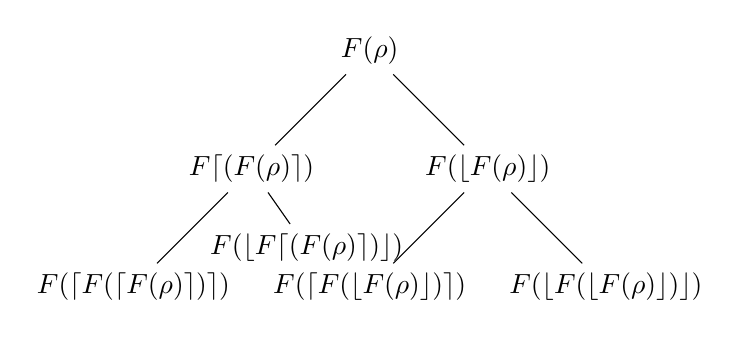
\begin{tikzpicture}
					\node {$F(\rho)$} [sibling distance = 3cm]
					child {node {$F\lceil(F(\rho)\rceil)$} 
						child {node {$F(\lceil F(\lceil F(\rho)\rceil)\rceil)$}}
						child {node [yshift = 0.5cm, xshift = -0.8cm]{$F(\lfloor F\lceil(F(\rho)\rceil)\rfloor)$}}}
					child {node {$F(\lfloor F(\rho)\rfloor)$}
						child {node {$F(\lceil F(\lfloor F(\rho)\rfloor)\rceil)$}}
						child {node {$F(\lfloor F(\lfloor F(\rho)\rfloor)\rfloor)$}
						}
					};
				\end{tikzpicture}
				\caption{GGM tree example to secretly share a value $x$ using a PRF $F$. $\lceil F(\rho)\rceil$ (resp. $\lceil F(\rho)\rceil$) denotes the first (resp. second) half of the output of $F(\rho)$.}
				\label{fig:GGMtree}
			\end{center}
		\end{figure}
		
		One challenge in this approach is the need to communicate the offset to the verifier so that they can verify the computations. However, a recent technique called \emph{Correlated GGM} (cGGM) has been introduced in \cite{GYWZ+22}, which allows the prover to generate random values $x^{\lir}$ using a modified GGM tree, such that $\sum_{i=1}^{N} x^{\lir} = x$, with no computational.
		This is achieved by enforcing an invariant over the cGGM tree: at each level, the sum of the nodes remains constant. More precisely, given a parent node $x$, the left child is defined as $F(x)$ and the right child as $x - F(x)$, where $F$ is a cryptographic psuedorandom function. As a result, only approximately half of the tree nodes require PRF evaluations, compared to all nodes in the classical GGM construction.
		This technique not only reduces the computational cost but also eliminates the need to transmit the offset to the verifier, thereby improving the overall communication efficiency.
		
		\begin{figure}[H]
		\begin{center}
			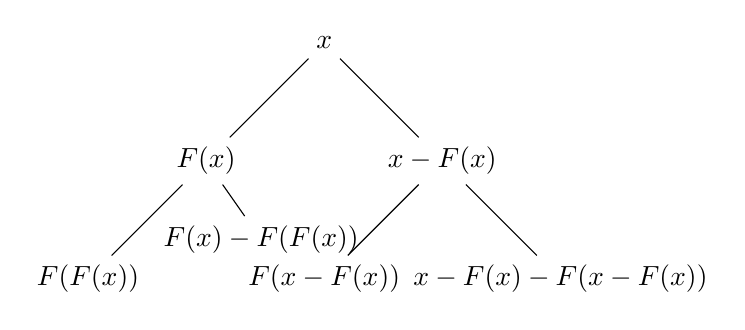
\begin{tikzpicture}
				\node {$x$} [sibling distance = 3cm]
				child {node {$F(x)$} 
					child {node {$F(F(x))$}}
					child {node [yshift = 0.5cm, xshift = -0.8cm]{$F(x) - F(F(x))$}}}
				child {node {$x - F(x)$}
					child {node {$F(x - F(x))$}}
					child {node {$x - F(x) - F(x -F(x))$}
					}
				};
			\end{tikzpicture}
			\caption{cGGM tree example. Here, it is easy to verify that the sum at each level is equal to $x$.}
			\label{fig:cGGMtree}
		\end{center}
		\end{figure}
		
		In practice, most MPCitH schemes use hash functions with a salt value but the size of the entry must be $2\lambda$ to achieve $2^{\lambda}$ security bits. A recent work by Bui et al. studied the security of using the AES as the PRF. specially because of it's hardware implementation which enables much faster tree generation than other PRF like SHA256 or other hash functions. The security of AES as a cryptographic PRF in a GGM tree generation has been studied in \cite{BCCG+24}. Thanks to AES hardware implementation like Intel's AES-NI instruction set, schemes can be up to 50x times faster than versions using hash functions like SHA256.
		
		\subsubsection{HyperCube technique}
 		This optimization technique was introduced in \cite{AGHH+22} and is commonly used in MPCitH schemes. This geometric approach models the $N$ shares as forming a $d$-dimensional hypercube of side length $k$. The often used parameters are $k = 2$ and $N = 2^d$, so the number party counts reduces to $log(N) + 1$. This technique often leads to MPC computations less expensive, smaller proof sizes and larger party sizes. However, these benefits come at the cost of increased reliance on GGM tree generation, which can become computationally expensive.
		
		\subsection{SBC Problem}
		The problem is the following: let $q$ be a prime power and two positive integers $k$, $n$.
		\newline
		Given two vectors $\vec{u}, \vec{v} \in (\mathbb{F}_{q^k})^n$, which are linearly independent over $\mathbb{F}_q$, find two non-colinear vectors $\vec{x}, \vec{y} \in (\mathbb{F}_q)^n$ such that $$(\vec{u} \cdot \vec{x})(\vec{v} \cdot \vec{y}) = (\vec{u} \cdot \vec{y})(\vec{v} \cdot \vec{x})$$
		where $(\cdot)$ is the dot product between 2 vectors.
		We denote an instance of the SBC problem given by two vectors $\vec{u}, \vec{v} \in (\mathbb{F}_{q^k})^n$ by $\text{SBC}[\vec{u}, \vec{v}]$. If the vectors $\vec{x},\vec{y} \in (\mathbb{F}_q)^n$ are solution of $\text{SBC}[\vec{u},\vec{v}]$, we use the notation $(\vec{x}, \vec{y}) \in \text{SBC}[\vec{u}, \vec{v}]$.
		
		\textbf{NSBC variant}.
		The authors also introduce a particular version of this problem called normalized SBC (NSBC) where $\vec{x}, \vec{y} \in (\mathbb{F}_q)^n$ and
		$\vec{x} = (\vec{x'}, 1, 0), \vec{y} = (\vec{y'}, 0, 1)$ to ensure that they are not colinear without needing to regenerate each time they are not. We also denote $(\vec{x}, \vec{y}) \in \text{NSBC}[\vec{u}, \vec{v}]$ if $(\vec{x}, \vec{y})$ are solutions to the NSBC problem on $(\vec{u}, \vec{v})$.
		
		\textbf{Key generation}. The private key $(\vec{x}, \vec{y})$ is constructed as such: uniformly at random choose $\vec{x'}, \vec{y'} \in (\mathbb{F}_q)^{n-2}$ and set $\vec{x} = (\vec{x'}, 1, 0)$ and $\vec{y} = (\vec{y'}, 0, 1)$.
		For the public key, randomly choose $\vec{u} \in (\mathbb{F}_{q^k})^{n}$ and $v_1,\dots,v_{n-1} \in \mathbb{F}_{q^k}$.
		Finally, set $v_n$ as:
		$$
			v_n = \frac{(\vec{u} \cdot \vec{y})(\sum_{i=1}^{n-1}v_ix_i) - (\vec{u} \cdot \vec{x})(\sum_{i=1}^{n-1}v_iy_i)}{y_n(\vec{u} \cdot \vec{x})}.
		$$
		
		\subsection{Keys and parameters estimations}
		The public key of this signature scheme is $(\vec{u},\vec{v})$ and the private key is $(\vec{x}, \vec{y})$.
		The signature and verification protocol use the MPCitH paradigm, they are described in detail in \cite{HJ23} with proof of soundness, correctness and zero-knowledge.
		The authors estimate that a good parameter for NSBC problem to be computationally secure are $q = 2, n = 130, k = 257$ using complexity analysis of what they think is the best known cryptanalysis of such problem on a classical computer in \cite{FSS11} with $\mathcal{O}(2^{354})$ operations. For the quantum cryptanalysis the estimate that the best attack would be using Grover's algorithm \cite{Grover} with $\mathcal{O}(n^{128})$ operations. 
		
		\subsection{Multiparty protocol for the SBC problem}
		
		
		
		\subsection{Identification Protocol}
		We present the identification protocol, which serves as a basis for constructing the signature scheme using the Fiat-Shamir transformation.
		
		\subsection{Keys and signature sizes}
		The size of the private key is just the size of the seed that is used to generate it which is derived from a PRF. So we only need to store the seed which is of size $\lambda$. So the size of the private key is $16$ bytes in practice. For the public key, we saw that all of it is generated randomly using a PRF and $v_n$ is computed. The size of $v_n$ is $2\lambda$ so the is size of public key is $3\lambda$ which in practice is $48$ bytes.
		
		The signature is composed of the following:
		\begin{itemize}
			\item One hash value $h$ corresponding to a global commitment to the $\tau$ round protocol of size $2\lambda$ and one salt of size $\lambda$.
			\item One punctured PRF key for each round.
			\item The valued $X_1+t_0(\vec{u}\dot\vec{x}), X_2+t_0(\vec{y}\dot\vec{x}) Y_1+t_0(\vec{v}\dot\vec{y}), Y_2+t_0(\vec{u}\dot\vec{y}) \in \mathbb{F}_{q^k}$ for each round.
		\end{itemize}
		The total size of the signature in bits is therefore
		$$
			\tau \dot (\lambda log_2(N)) + 10\tau \lambda + 3\lambda = \lambda^2 + 10 \tau \lambda + 3 \lambda \text{ bits},
		$$
		where we use the fact that $\lambda = \tau log_2(N)$ in the equation.
		We remind that we do not need to communicate the auxiliary values $\delta_A, \delta_B, \vec{\delta}_x$ and $\vec{\delta}_y$ if we use a correlated GGM tree.
		
	\section{Polynomial system solving}\label{sec3}
		Gröbner basis theory was first introduced by Buchberger in his thesis \cite{Buc} and he gave an algorithm to compute the Gröbner basis of an ideal.
		Gröbner basis algorithms like Buchberger's Algorithm \cite{Buc}, are used to find solutions for polynomial systems using algebraic geometry tools. For a gentle introduction to this subject \cite{CLS}.
		
		In \cite{Lazard83}, Lazard introduced the connection between linear algebra and Gröbner basis theory via the usage of Macaulay matrices \cite{Mac} which is defined as follows.
		
		\begin{definition}
			Let $\prec$ be an admissible monomial ordering on a given ring $R$. Given a sequence of homogeneous (resp. affine) polynomials $\mathcal{F} = (f_1,\dots,f_m) \in R$, we associate to it the Macaulay matrix of degree $D$ (resp. $\leq D$), denoted by $\Mac{D}{m}{\mathcal{F}}$ (resp. $\Mac{\leq D}{m}{\mathcal{F}}$), and defined as follows: the columns of the matrix are indexed by the monomials of degree $D$ (resp. $\leq D$) sorted in decreasing order from the left to right using the defined monomial ordering. Each row of the matrix is labeled by a tag, also called signature, ($u, f_i$) where u is a monomial in $R$ and $f_i \in \mathcal{F}$ such that $deg(uf_i) = D$ (resp. $deg(uf_i) \leq D$), and the polynomial $uf_i$ is written as vector of coefficients of monomials on the row. We denote by $\Mact{D}{m}{F}$ (resp. $\Mact{\leq D}{m}{F}$) the row echelon form of $\Mac{D}{m}{\mathcal{F}}$ (resp. $\Mac{\leq D}{m}{\mathcal{F}}$) without swapping columns to preserve the monomial ordering.
		\end{definition}
		
		\subsection{Faugère's F5}
		
		The major "issue" of Gröbner basis algorithms like Bucherberger's \cite{Buc}, F4 \cite{F02} are the reductions to 0 in the Macaulay matrix associated to a polynomial sequence $\Mac{D}{m}{F}$, because the size of the matrices are huge, multiple millions rows and columns for practical examples,
		reductions to 0 can cost a lot during the linear algebra process. F5 \cite{F02} was a major improvement because it provided a criterion that avoided reduction to 0 during the linear algebra part for all regular sequences.
		
		\begin{proposition}[General criterion \cite{F02}]
			\label{F5Crit}
			Let $d_i$ be the total degree of $f_i \forall i \in [1,m]$.
			$\forall j < m$, if a row of signature ($u, f_j$) in the matrix $\Mact{D-d_j}{m-1}{F}$ has as leading term $t'$, then the row ($t', f_m$) in $\Mac{D}{m}{F}$ (resp. $\Mac{\leq D}{m}{F}$) will reduce to 0 i.e. is a linear combination of the predecessors.
		\end{proposition}
		
		\begin{proposition}[Frobenius criterion \cite{F02}]
			\label{Frob}
			If a row of signature ($t, f_m$) in $\Mact{D - d_m}{m}{F}$ has as leading term $t'$, then the row ($t', f_m$) in $\Mac{D}{m}{F}$ (resp. $\Mac{\leq D}{m}{F}$) will reduce to 0.
		\end{proposition}
		
		The Frobenius criterion \ref{Frob} is the analogue of the General criterion \ref{F5Crit} but for polynomial systems defined over $\mathbb{F}_2$.
		F5 criterion and Frobenius criterion remove the rows corresponding to the trivial syzygies, i.e. the syzygies $(s_1, \dots, s_m)$ such that for a row with signature $(s_i, f_i)$, we get $s_i \in \langle f_1,\dots,f_{i-1},f_{i+1},\dots,f_m \rangle$.
		
		Bardet introduced a variant of F5 Algorithm that is simple to understand and analyze called Matrix F5 in \cite{Bardet04}.
		We give the description of Matrix F5 Algorithm.
		
		\begin{algorithm}
			\caption{Matrix F5}\label{alg:matrix_f5}
			\begin{algorithmic}[1]
				\Require 
				\begin{tabular}[t]{@{}l@{}}
					$\left\{ 
					\begin{array}{l}
						m \text{ homogeneous polynomials } f_1, \dots, f_m \text{ of degree } d_1 \leq d_2 \leq \dots \leq d_m, \\
						D \text{ an integer}, \\
						\text{a monomial ordering } \prec
					\end{array}
					\right.$
				\end{tabular}
				\Ensure 
				\begin{tabular}[t]{@{}l@{}}
					$\left\{ 
					\begin{array}{l}
						G \text{ is a Gröbner basis of } \langle f_1,\dots,f_m \rangle.
					\end{array}
					\right.$
				\end{tabular}
				\State $G \gets {f_1,\dots,f_m}$
				\For{$d$ from $d_1$ to $D$}
					\State $\widetilde{Mac}_{d, 0} \gets$ matrix with 0 rows
					\For{$i$ from $1$ to $m$}
						\State Construct ${Mac}_{d, i}$ by adding to $\widetilde{Mac}_{d, i-1}$ the following rows:
						\If{$d_i = d$}
							\State Add the row $f_i$ with signature $(1, f_i)$
						\EndIf
						\If{$d > d_i$}
							For all $f$ from $\widetilde{Mac}_{d, i-1}$ with signature $(e, f_i)$, such that $x_\lambda$ is the greatest variable of $e$, add the $n - \lambda + 1$ rows $x_\lambda f,x_{\lambda + 1}f,\dots,x_n f$ with the signatures $(x_\lambda e, f),(x_{\lambda + 1}e, f),\dots,(x_n e, f)$ except those who satisfy the F5 criterion with $((x_{\lambda + k}e, fi), \widetilde{Mac}_{d-d_i, i-1}$
						\EndIf
						\State Compute $\widetilde{Mac}_{d, i}$ the row echelon form of ${Mac}_{d, i}$
						\State Add to $G$ the polynomials corresponding to the rows of $\widetilde{Mac}_{d, i}$ such that their leading
						\State monomials is different from the leading monomial of the row with the
						\State same signature in ${Mac}_{d, i}$
				 	\EndFor
				\EndFor
				\State \textbf{Return} $G$
			\end{algorithmic}
		\end{algorithm}
		
		\subsection{Hilbert series}
		Hilbert-Poincaré series (or Hilbert series) is a very important tool in algebraic geometry to describe ideals, varieties and their dimensions.
		\begin{definition}[\cite{CLS}]
			Let $I$ be a homogeneous ideal in $R$. The affine Hilbert function of $I$ is the function on the nonnegative integers is defined by
			$$
				{}^a HF_{R/I}(s) = dim R_{s} / dim I_{s} = dim R_{s} - dim I_{s}.
			$$
		\end{definition}
		
		\begin{proposition}
			${}^a HF_{R/I}(s)$ is the number of monomials not in $I$ of total degree $s$.
		\end{proposition}
		\begin{proof}
			First note that the monomials ${x^\alpha | \alpha \leq s}$ is a basis of $R_{\leq s}$ as a vector space. We also have that ${x^\alpha | \alpha \leq s | x^\alpha \in I}$ is a basis of $I_{\leq s}$. Therefore, the monomials ${x^\alpha | \alpha \leq s | x^\alpha \notin I}$ are the ones missing to form a basis for $R$, so they form a basis for $R_{\leq s} / I_{\leq s}$ which concludes the proof.
		\end{proof}
		
		\begin{definition}
			Let I be a homogeneous ideal. The Hilbert series is defined as follows
			$$
					HS_{R/I}(t) = \sum_{m=0}^{\infty} HF_{R/I}(m) t^m.
			$$	
		\end{definition}
		
		The index of regularity is the smallest integer $s_0$ such that $HF_{R/I}(s_0)$ is equal to a certain polynomial called the Hilbert polynomial. It is also the smallest integer $s_0$ such that the coefficient of the Hilbert series is less or equal to 0. We will denote $H(I)$ as the index or degree of regularity of I.
		
		Faugère showed that no reductions to 0 occur in the Macaulay matrix during the F5 algorithm \ref{alg:matrix_f5} until the degree of regularity \cite{F02} for regular sequences.
		
		\subsection{Semi-regularity}
		One problem with the definition of a regular sequence, is that it applies for only underdetermined  polynomial systems because on of the properties of a regular sequence of a polynomial system $f_1,\dots,f_m \in \mathbb{K}[x_1,\dots,x_n]$ is that the dimension of the ideal $\langle f_1,\dots,f_m \rangle$ is $n - m$. This property can not be verified for overdetermined systems because the dimension of the ideal can not be negative.
		
		Thus, Bardet studied a new concept called semi-regularity for overdetermined system to allow their study and analysis. The definition of a semi-regular sequence is given by Bardet \cite{Bardet04}.
		
		\begin{definition}
			A zero-dimensional homogeneous sequence $f_1,\dots,f_m \subset R$ is semi-regular if the following conditions are verified:
			\begin{itemize}
				\item $I = \langle f_1,\dots,f_m \rangle \neq R$,
				\item For $i \in [1:m]$, if $g_if_i = 0$ in $R/\langle f_1,\dots,f_m \rangle$ and $deg(g_if_i) < H(I)$ then $g_i = 0$ in $R/\langle f_1,\dots,f_m \rangle$.
			\end{itemize} 
		\end{definition}
		
		Bardet also showed that if we apply matrix-F5 \ref{alg:matrix_f5} to a semi-regular system, there are no reductions to 0 until the degree $d = H(I) - 1$. We also have a certain reciprocity.
		
		One interesting thing shown by Bardet \cite{Bardet04}, is that a random polynomial system is very likely to be semi-regular. Most of the cryptosystems using random polynomial systems assume the semi-regularity of the system to ease their analysis using well established tools. For example, one can compute the Hilbert series of a semi-regular system easily.
		
		\begin{proposition}[Proposition 3.2.5 in \cite{Bardet04}]\label{PropSemi}
			Let $f_1,\dots,f_m$ a semi-regular homogeneous sequence, $f_i$ is of degree $d_i$. Then the following properties are verified:
			\begin{itemize}
				\item The sequence $f_1,\dots,f_m$ is semi-regular if and only if its Hilbert series is the series $$S_{m, n}(z) = \sum_{d \geq 0}h_{d, m}(n)z^d = \prod_{i=1}^{m}(1-z^{d_i})/(1-z)^n.$$ $S_{m, n}(z)$ is called the generating series of $f_1,\dots,f_m$.
				\item The sequence $f_1,\dots,f_m$ is semi-regular on $\mathbb{F}_2$, if and only if its Hilbert series is the series $$S_{m, n}(z) = \sum_{d \geq 0}h_{d, m}(n)z^d = (1+z)^n/\prod_{i=1}^{m}(1+z^{d_i}).$$ $S_{m, n}(z)$ is called the generating series of $f_1,\dots,f_m$.
				\item Every permutation $f_{\sigma(1)},\dots,f_{\sigma(m)}$ is a semi-regular sequence.
				\item When the associated variety is zero-dimensional, $H(I)$ is characterized by
				$$
				\forall d < H(I), h_{d, m}(n) > 0 \text{ and } h_{H(I), m}(n) \leq 0.
				$$
				\item The sequence $f_1,\dots,f_m$ is semi-regular $\nRightarrow \forall i \in [1;m]$, the sequence $f_1,\dots,f_i$ is semi-regular. 
			\end{itemize}
		\end{proposition}
		
		\subsection{Bilinear systems case}
		Our NSBC instances are quadratic systems that are bilinear in the variables of degree 2 and overdetermined.
		
		\begin{definition}
			A homogeneous polynomial $f \in \mathbb{K}[x_1,\dots,x_{n_x},y_1,\dots,y_{n_y}]$ is called bilinear if we have:
			$$
			\forall \lambda, \mu \in \mathbb{K}, f(\lambda x_1,\dots,\lambda x_{n_x}, \mu y_1,\dots, \mu y_{n_y}) = \lambda \mu f(x_1,\dots,x_{n_x},y_1,\dots,y_{n_y}).
			$$
		\end{definition}
		
		A bilinear system is a polynomial system where each equation is a bilinear form.
		
		We will denote $n_x$ (resp. $n_y$) the number of variables in $x$ (resp. in $y$). In our case, $n_x = n_y = (m-1)/2$ and $m = k$.
		
		The article \cite{FSS11} and the thesis \cite{Spaen2012} provide a new criterion for bilinear determined systems and a complexity analysis of their algorithm (the proofs in the end of \cite{FSS11} are not exact, the authors recommended to refer to \cite{Spaen2012} for better proofs) that removes all reductions to 0 in F5 Algorithm for bilinear systems which are not semi-regular.
		
		\subsubsection{Jacobian matrices and syzygies}
		First we will need to introduce some important notations.
		\begin{itemize}
			\item[-] Let $f_1,...,f_m \in R$ be a bilinear polynomial. We denote by $F_i$ the polynomial sequence $(f_1,...,f_i)$ and $I_i$ the ideal spanned by this sequence $\langle F_i \rangle$.
			\item[-] $jac_{x}(F_{i-1})$ (resp. $jac_{y}(F_{i-1})$) is the jacobian matrix with respect to the two subsets of variables $x_1,...,x_{n_x}$ (resp. $y_1,...,y_{n_y}$).
			\item[-] Let $M$ be a $l \times c$ matrix with $l > c$. We call maximal minors of $M$ the determinants of the $c \times c$ sub-matrices of $M$. We denote the maximal minors of $M$ by $MaxMinors(M)$.
			\item[-] $I_{i-1} : f_i$ is the ideal spanned by $\{g \in R \mid gf_i \in I_{i-1}\}$.
		\end{itemize}
		We will give important results of this article before discussing them further.
		
		\begin{theorem}[Theorem 2 in \cite{FSS11}]\label{theoremMaxMin}
			Let $i > n_x + 1$ (resp. $i > n_y + 1$) and let $s$ be a linear combination of maximal minors of $jac_{x}(F_{i-1})$ (resp. $jac_{y}(F_{i-1})$). Then $s \in I_{i-1} : f_i$.
		\end{theorem}
		
		As Theorem \ref{theoremMaxMin} indicates, reductions to 0 may also arise from the maximal minors of the jacobian matrix, so the signatures ($s, f_i$) where $s$ is a linear combination of maximal minors of $jac_{x}(F_{i-1})$ or $jac_{y}(F_{i-1})$ is a reduction to 0.
		This explains Algorithm \ref{alg:crit_calc} where we compute the maximal minors of jacobian matrices before applying Algorithm \ref{alg:reduc} where we compute linear combinations of these maximal minors.
		This means that Algorithm \ref{alg:crit_calc} computes all the signatures that will arise in reductions to 0 that involve the maximal minors of jacobian matrices instead of being incremental like F5 criterions \cite{F02}.
		
		\begin{algorithm}
			\caption{Reduce}\label{alg:reduc}
			\begin{algorithmic}[1]
				\Require A monomial ordering $\prec$ and $S$ a set of homogeneous polynomials and $q$ a degree.
				\Ensure $T$ a reduced set of homogeneous polynomials of degree $q$.
				\State $M \gets Mac_{\prec}(S, q)$.
				\State $M \gets RowEchelonForm(M)$.
				\State \textbf{Return} $T$ the set of polynomials corresponding to the rows of M.
			\end{algorithmic}
		\end{algorithm}
		
		\begin{algorithm}
			\caption{BL\_Criterion}\label{alg:crit_calc}
			\begin{algorithmic}[1]
				\Require $m$ bilinear polynomials $f1,...f_m$ such that $m \leq n_x + n_y$.\newline $\prec$ a monomial ordering overs $R$.
				\Ensure $V$ a set of pairs $(h, f_i)$ such that $h \in I_{i-1} : f_i$ and $h \notin I_{i-1}$.
				\State $V \gets \emptyset$
				\For{$i$ from 2 to $m$}
				\If{$i > n_y$}
				\State $T \gets \mathbf{Reduce}(MaxMinors(jac_y(F_{i-1})), n_y + 1)$
				\For{$h$ in $T$}
				\State $V \gets V \cup \{(h, f_i)\}$
				\EndFor
				\EndIf
				\If{$i > n_x$}
				\State $T' \gets \mathbf{Reduce}(MaxMinors(jac_x(F_{i-1})), n_x + 1)$
				\For{$h$ in $T'$}
				\State $V \gets V \cup \{(h, f_i)\}$
				\EndFor
				\EndIf
				\EndFor
				\State \textbf{Return} $V$
			\end{algorithmic}
		\end{algorithm}
		
		\begin{algorithm}
			\caption{BilinF5Criterion}\label{algo:crit}
			\begin{algorithmic}[1]
				\Require $(t, f_i)$ the signature of a row. \newline A matrix $M$ in row echelon form.
				\Ensure $True$ if the row will reduce to 0 otherwise $False$.
				\If{$t$ is the leading monomial of a row of $M$ \textbf{or}
					\newline $\exists (h, f_i) \in V$ such that $LM(h) = t$}
				\State \textbf{Return} $True$.
				\Else \textbf{ Return} $False$.
				\EndIf
			\end{algorithmic}
		\end{algorithm}
		
		\begin{definition}[Definition 8 in \cite{FSS11}]
			Let $\prec$ be a monomial ordering such that its restriction to $\mathbb{K}[x_1,\dots,x_{n_x}]$ (resp. $\mathbb{K}[y_1,\dots,y_{n_y}]$) is the grevlex ordering. Let $m \leq n_x + n_y$ and $f_1,\dots,f_m$ be bilinear polynomials or $R$. We say that the polynomial sequence ($f_1,\dots,f_m$) is a \textit{bi-regular} sequence if $m = 1$ or if ($f_1,\dots,f_m$) is a \textit{bi-regular} sequence and
			$$
			LM(I_{m-1} : f_m) = \langle Monomials_{m - n_y - 2}^x(n_y + 1) \rangle + \langle Monomials_{m - n_x - 2}^y(n_x + 1) + LM(I_{m-1})\rangle.
			$$
		\end{definition}
		
		We can notice that the output of algorithm \ref{alg:reduc} is polynomials of degree $q$. Here $q$ is always $n_x + 1$ or $n_y + 1$. We deduce that the only non trivial syzygies are of degree $n_x + 1$ or $n_y + 1$. \textbf{c'est pas $n_x + 2$ ou $n_y + 2$ du coup ?}
		
		The following theorem, ensures that there are no reductions to 0 with extended the F5 criterion. \textbf{Ce théorème est en suspens pour utiliser une autre formulation sans utiliser la topologie de Zariski}
		
		\begin{theorem}[Theorem 4 in \cite{FSS11}]
			Let $m, n_x, n_y \in \mathbb{N}$ such that $m < n_x + n_y$. If Conjecture 1 of \cite{FSS11} is true, then the set of bi-regular sequences $(f_1,...,f_m)$ contains a nonempty Zariski open set. Moreover, if $(f_1,...,f_m)$ is a bi-regular sequence, then there are no reductions to zero with the extended F5 criterion.
		\end{theorem}
		
		An important result of \cite{FSS11} is on the index of regularity of bi-regular systems.
		
		\begin{theorem}\label{reg_bi}
			If the system $\mathcal{F}$ is a generic bilinear system, then the degree of regularity of $\mathcal{V}(I)$ is upper bounded by $d_{reg} \leq min(n_x, n_y)$.
		\end{theorem}
		
		Finally, the authors give the following corollary which is the consequence of \ref{reg_bi} by applying the complexity of computing a Gröbner basis given by \cite{Bardet04}.
		
		\begin{corollary}[Corollary 3 in \cite{FSS11}]\label{complex_bi}
			The arithmetic complexity of computing a Gröbner basis of a generic affine bilinear system $f_1,...,f_{n_x + n_y}$ with the F5 algorithm is bounded by
			$$\mathcal{O}\left(\binom{n_x + n_y + min(n_x + 1, n_y + 1)}{min(n_x + 1, n_y + 1)}^\omega\right).$$
		\end{corollary}
		
		\begin{corollary}
			
		\end{corollary}
		
		First, we can clearly see that the complexity of Algorithm \ref{alg:crit_calc} is exponential and we will show that in the following proposition.
		
		\begin{proposition}\label{complexCrit}
			The complexity of Algorithm \ref{alg:crit_calc} is
			$$
			\mathcal{O}\left(\left(\sum_{i = n_x}^{m} \binom{i}{n_x}n_x^{\omega} + \binom{2n_x + 1}{n_x}^\omega\right) + \left(\sum_{i = n_y}^{m} \binom{i}{n_y}n_y^{\omega} + \binom{2n_y + 1}{n_y}^\omega\right)\right).
			$$
		\end{proposition}
		
		\begin{proof}
			First, if $i > n_y$ (resp. $i > n_x$), we construct the jacobian matrix $jac_y(F_{i-1})$ (resp. $jac_x(F_{i-1})$) which is of size $n_y \times n_y$ (resp. $n_x \times n_x$) for the first one and $m-1 \times n_y$ (resp. $m-1 \times n_x$) for the last one i.e. $i = m$. We suppose here that the construction of such matrices is free. Computing the $MaxMinors(jac_y(F_{i-1}))$ (resp. $MaxMinors(jac_x(F_{i-1}))$)means that we have to compute the determinants of all the sub-matrices of size $n_y \times n_y$ (resp. $n_x \times n_x$) and for a matrix $M$ of size $l \times c$ with $l > c$ there are $\binom{l}{c}$ sub-matrices of size $c \times c$, hence the term $\binom{i}{n_y}n_y^{\omega}$ in the sum if we suppose the complexity of computing the determinant of a square multivariate polynomial matrix of size $c \times c$ to be $\mathcal{O}(c^\omega)$, which is not the case but let us suppose the best case ever. \textbf{faudrait trouver la vraie complexité de ça pour être plus juste.}
			For now, we have a sequence of polynomials and we apply the algorithm \textbf{Reduce} \ref{alg:reduc} on them with degree $n_y + 1$ (resp. $n_x + 1$).
			In \textbf{Reduce}, we construct the Macaulay matrix of the sequence of degree $n_y + 1$ (resp. $n_x + 1$) and compute it's row echelon form.
			The size of Macauly matrix is bounded by $\binom{n + D}{D}$ where D is the degree and n the number variables. So the complexity of \textbf{Reduce} is $$\mathcal{O}\left(\binom{n_y + n_y + 1}{n_y + 1}^\omega \right)$$ (resp. $$\mathcal{O}\left(\binom{n_x + n_x + 1}{n_x + 1}^\omega \right)$$). Hence the second term in the sum, because we call \textbf{Reduce} at each iteration of the for loop. We finally suppose that the iteration on the elements of the output of \textbf{Reduce} is negligible in the big $\mathcal{O}$ notation.
		\end{proof}
		
		It is an asymptotic complexity which does not take into account the constant factor in implementations that could slow down a lot the algorithm.
		We also recall that in our case with NSBC, $n_x = n_y$. So we get
		$$
		\mathcal{O}\left(2n_x^{\omega}\left(\sum_{i = n_x}^{m} \binom{i}{n_x} + \binom{2n_x + 1}{n_x}^\omega\right)\right).
		$$
		
		Since we have quadratic systems, reductions to 0 would not appear before degree 4 of the Macaulay matrix. Also, in practice we are using $q=2$ and there are much better algorithms in the literature for boolean systems than basic Gröbner basis algorithms like F5. The best algorithm used at the moment is CrossBred \cite{JV17}. Most of the time in practical implementations, we stop at degree 4 of the Macaulay in pre-processing step. So, to know what advantage we could have if we use the extended F5 criterion, we will suppose the worst, meaning that all of our entries will reduce to 0 at degree 4 of the Macaulay matrix, which is unlikely.
		
		In following, we will denote $n_x + n_y$ by simply $n$.
		
		If this case arises, the only computations that would be done are for extended F5 criterion. The complexity for F5-Matrix algorithm with only the Frobenius criterion \ref{Frob} is 
		$$
		\mathcal{O}\left(\binom{n + 4}{4}^\omega\right).
		$$
		If we only take into consideration the big O notation and not the constants, which is not realistic at all for efficient implementations to really break a cryptographic scheme, we get
		\begin{equation}
			Adv(n, m) = 2\left(\sum_{i = n/2}^{m}\binom{i}{n/2}\left(\frac{n}{2}\right)^\omega + \binom{n + 1}{n/2}^\omega\right) - \binom{n + 4}{4}^\omega.
			\label{equation_complex}
		\end{equation}
		
		We used the computer algebra system SageMath \cite{sagemath} to test numerically when using the F5 extended criterion of \cite{FSS11} becomes negligible compared to the computations of reductions to 0, we see experimentally that $Adv(10, 12) = 2498903$, i.e. the theoretical advantage becomes negligible and it would be advantageous to simply compute reductions to 0 instead of applying the F5 extended criterion. This number grows exponentially with $n$ and $m$. For those who wonder, what would be the estimated theoretical advantage computing reductions to 0 for the parameters given by \cite{HJ23} $Adv(256, 257)$ is a 514 bit number.
		
		\subsection{Boolean systems}
		Sometimes, the finite field used is $\mathbb{F}_2$ because it is still supposedly hard to solve but is very easy to use and manipulate on computers. But in such small fields one can begin to use exhaustive search to obtain the solution to the system. The best algorithm known to the authors for exhaustive search for multivariate polynomial system $f_1,\dots,f_m$ over $\mathbb{F}_2[x_1,\dots,x_n]$ is \cite{BCC+10} with a complexity $\mathcal{O}(ln(n)2^n)$. What is remarkable is that the complexity does not implicate the number of polynomials in the system, $m$. There is also a software made by one of the authors, Charles Bouillaguet, that is available online and easy to use, \textit{libFES-lite} \cite{Bouilla22} and there have been implementations on FPGA that broke real world cryptography \cite{DDVY20}..
		
		Another type of algorithms uses exhaustive search combined with probabilistic algorithms. \cite{LPT+17} gave an algorithm that finds the solution to a polynomial system with complexity $\tilde{\mathcal{O}}(2^{0.8765n})$ which is better than exhaustive search. Even though it is asymptotically better, there are no known implementations because of the huge constant factors present in the complexity that makes it worse than exhaustive search for any systems that can be solved on modern computers. New algorithms have been proposed by Itai Dinur \cite{Itai21A, Itai21B} where the complexity is brought down to $\tilde{\mathcal{O}}(2^{0.6943n})$, but still no implementation known to the authors.
		
		The last type is a hybrid algorithms using Gröbner basis algorithms and exhaustive search to find solutions. The most known and the best one is BooleanSolve hybrid by Bardet, Faugère, Salvy and Spaenlehauer \cite{BFSS13} where we guess a certain number of variables $k$ and apply F5 algorithm on the specialized systems. Under semi-regularity assumption, the algorithm finds the solution in $\mathcal{O}^(2^{0.792n})$ if $n = m$ and $k = 0.55n$. This is better than exhaustive search, but still, the constant factors are too big for it to be better for systems smaller with less than 200 variables.
		
		The algorithm on which I focused on during my internship is Crossbred by Joux and Vitse \cite{JV17}. It mixes the usage of exhaustive search and algebraic algorithms like BooleanSolve hybrid but with a pre-processing step before doing the exhaustive search and applying algebraic algorithms like XL \cite{CKPS00} or it's variants or F5 \cite{F02}.
		
		To understand this algorithm, we will need definitions of special Macaulay matrices used by it.
		
		We will denote by $deg^k(p)$ the total degree of $p$ in the first $k$ variables.
		
		\begin{definition}
			For a given $\mathcal{F} = \{f_1,\dots,f_m\}$, $Mac_{\leq D, \geq d, m}^k$ is the submatrix of $Mac_{\leq D, m}$ whose rows correspond to a product $uf_i$, $1 \leq i \leq m$, with $deg^k(u) \geq d-1$. Let $\mathcal{M}_{\leq D, \geq d, m}^k$ be the submatrix of $Mac_{\leq D, \geq d, m}^k$ with columns correspond to monomials $m$ such that, $deg^k(m) \geq d+1$.
		\end{definition}
		
		\begin{algorithm}
			\caption{The CrossBred algorithm}\label{alg:crossbred}
			\begin{algorithmic}[1]
				\Require Polynomials $\mathcal{F} = {f_1, \dots, f_m}$ of $n$ variables and integers $D,d,k$
				\Ensure  A solution for the system if it exists or nothing otherwise.
				\State Construct $Mac_{\leq D, \geq d, m}^k(\mathcal{F})$ and $\mathcal{M}_{\leq D, \geq d, m}^k(\mathcal{F})$
				\State Compute a basis $(v_1,\dots,v_r)$ if the left kernel of $\mathcal{M}_{\leq D, \geq d, m}^k(\mathcal{F})$
				\State Construct the polynomials $p_1,\dots,p_r$ corresponding to $v_i \cdot Mac_{\leq D, \geq d, m}^k(\mathcal{F})$.
				\For{$a = (a_{k+1},\dots,a_n) \in \mathbb{F}_{2}^{n-k}$}
				\State Evaluate the last $n-k$ variables in each $f_i \in \mathcal{F}$ at $(a_{k+1},\dots,a_n)$ and compute $\mathcal{F}*$
				\State Compute $Mac_{\leq d, m}(\mathcal{F}*)$
				\State Compute $\mathcal{F}'*$ as the partial evaluation of $F' = {p_1,\dots,p_r}$ at $(a_{k+1},\dots,a_n)$
				\State Consider the system $S*$ consisting of $Mac_{\leq d, m}(\mathcal{F}*) \cup \mathcal{F}'*$
				\If{$S*$ is consistent using XL for example}
				\State \textbf{Return} solution
				\EndIf
				\EndFor
			\end{algorithmic}
		\end{algorithm}
		
		This algorithm have shown it's effectiveness in practice with good implementations like Bouillaguet and Sauvage's implementation \cite {BS23} that broke records for solving boolean systems on the Fukuaka MQ challenge \cite{MQFUK}. Despite that, there are no proven complexity analysis for this algorithm due to it's huge number of possible parameters but we can do some estimations with admissible parameters as we will see in the next section.

	\section{Contributions}\label{sec4}
		
		\subsection{System Modeling}
		One of the known attacks given by the authors is through algebraic cryptanalysis.
		One can model the attack by taking $g$ as the following polynomial
		$$
		g(x_1,...,x_n,y_1,...,y_n) := (\vec{u} \cdot \vec{x})(\vec{v} \cdot \vec{y}) - (\vec{u} \cdot \vec{y})(\vec{v} \cdot \vec{x}).
		$$
		We consider
		$$
		g(x_1,..,x_{n-2},y_1,..,y_{n-2}) := (\sum_{i = 1}^{n-2}u_{i}x_{i} + u_{n-1})(\sum_{i = 1}^{n-2}v_{i}y_{i} + v_{n}) - (\sum_{i = 1}^{n-2}u_{i}y_{i} + u_{n})(\sum_{i = 1}^{n-2}v_{i}x_{i} + v_{n-1}).
		$$
		
		Then, one can perform a Weil descent on the polynomial $g$ because $\mathbb{F}_{q^k}$ is a $\mathbb{F}_q$-vector space and obtain the polynomial system
		
		
		\begin{align}
			g_1(x_1, \dots, x_{n-2},& y_1, \dots, y_{n-2}) = 0 \notag \\
			&\vdots \notag \\
			g_k(x_1, \dots, x_{n-2},& y_1, \dots, y_{n-2}) = 0 \notag
		\end{align}
		
		where $g_i$ are polynomials with coefficients in $\mathbb{F}_q$.
		
		The most straightforward cryptanalysis of this type of systems is to perform a Gröbner basis algorithm like Buchberger's algorithm \cite{Buc}, Faugère's F4 \cite{F99}, F5 \cite{F02} or their multiple variants \cite{EF19}.
		
		Huth and Joux cite a complexity result in \cite{FSS11} to argue their parameters choice, we will dive deeper into this article  results in a later section.
		
		\subsection{Algebraic cryptanalysis}
		
		Bardet showed in \cite{Bardet04} that F5 criterion removed reductions to 0 for semi-regular sequences until the degree $H(I) - 1$, where $I$ is the ideal generated by the polynomials of the system.
		
		\begin{theorem}[Theorem 3.2.10 in \cite{Bardet04}]
			Let $f_1,...,f_m$ a homogeneous sequence, such that $\langle f_1,...,f_m \rangle$ is 0-dimensional and
			$\prec$ an admissible graded monomial ordering. We have,
			\begin{itemize}
				\item[-] If the sequence is semi-regular, then no reductions to 0 are performed during the F5-matrix algorithm until the degree $d = H(I) - 1$
				\item[-] If there are no reductions to 0 during the F5-matrix algorithm until the degree $D - 1$, and if the matrix of degree D is full rank and is the first matrix to have more rows than columns, then the sequence is semi-regular and its index of regularity is $H(I) = D$.
			\end{itemize}
		\end{theorem}
		
		In \cite{BFS15}, the authors show that the complexity of computing the Gröbner basis of a semi-regular system $f_1,...,f_m \in \mathbb{K}[x_1,...,x_n]$ is $O\left(mD\binom{n+D-1}{D}^\omega \right)$.
		
		
		We will also need the next definition of $\gamma$-strong semi-regularity.
		
		 \begin{definition}[Definition 4 of \cite{VID24}]
			Let $\mathcal{F} = {f_1,...,f_m}$ be a semi-regular sequence of polynomials in $\mathbb{F}_2[x_1,...,x_n]$ and let $0 \leq \gamma \leq 1$ such that $k = (1 - \gamma)n$. We say that this sequence is $\gamma$-strong semi-regular if
			$$
			\mathcal{S}(I) = \{(a_{k+1},...,a_n) \in \mathbb{F}_{2}^{n-k} |
			$$
			$$
			\{f_1(x_1,...,x_k,a_{k+1},...,a_n),...,f_m(x_1,...,x_k,a_{k+1},...,a_n)\} \text{ is not semi-regular}\}
			$$
			has cardinality $\mathcal{O}(2^{-\gamma n})$.
		\end{definition}
		
	\subsection{Admissible parameters for Crossbred}
		We tested if small instances of our problem are semi-regular or not using Proposition \ref{PropSemi} and they were not semi-regular. We also remarked that the bilinear criterion \ref{algo:crit} detected reductions to 0 using the original F5 criterion \ref{F5Crit} and Frobenius criterion for systems over $\mathbb{F}_2$ but also detected reductions to 0 on polynomials of degree $n_x$ or $n_y$ according to the algorithms \ref{alg:crit_calc} and \ref{alg:reduc}. In our case, we will use the Crossbred algorithm and we do not think that we will get to these degrees in the Macaulay matrices, so no need to use the bilinear criterion.
		
		Even though no concrete complexity analysis is available for the Crossbred algorithm because of it's wide parameters choice, there are some articles that give formal tools to analyze admissible parameters and try to estimate the complexity for these parameters. We choose to focus on the article \cite{VID24} to select valid parameters and estimate the complexity of the algorithm using them.
		
		\begin{theorem}\label{serie_=H}
			Let $H_{m, n}^k(X,Y) = \sum_{d_1 \geq 0, d_2 \geq 0} h_{d_1, d_2, m}^k X^{d_1}Y^{d_2}$ be the bivariate series with coefficient which is the number of new "independent" polynomials generated during the pre-processing. This series is given by:
			$$
				H_{m, n}^k(X, Y) = \frac{1}{Y}\left((1+X)^{n-k} - \frac{(1+XY)^k(1+X)^{n-k}}{(1+X^2Y^2)^m}\right).
			$$
		\end{theorem}
		
		\begin{proposition}\label{serie_G}
			For fixed values of $m, n \text{ and } k$ the bivariate series $G^{k}_{m,n}(X, Y) = $ \\ $\sum_{d_1 \geq 0, d_2 \geq 0}(\sum_{d_{1}' \leq d_1, d_{2}' \geq d_2} g_{d_{1}',d_{2}',m}^k)X^{d_1}Y^{d_2}$ is given by the formula:
			$$
				G^{k}_{m,n}(X, Y) = - \frac{YH_{m, n}^k(X,Y) - H_{m, n}^k(X, 1)}{(1-X)(1-Y)}.
			$$
			the coefficient in front of $X^{d_1}Y^{d_2}$ is the number of polynomials generated during the pre-processing step for a given pair $(d_1, d_2)$.
		\end{proposition}
		
		We also have that by definition \( h_{d_1, d_2, m}^k \) is defined as:
		\begin{align}
			h_{d_1, d_2, m}^k =
			\begin{cases}
				U_{d_1, d_2, m}^k - M_{d_1, d_2 + 1}^k, & \text{if } d_1 \geq d_2 \geq 0,\ m \geq 1, \\
				- M_{d_1, 0}, & \text{if } d_1 \geq 0,\ d_2 = -1,\ m \geq 0, \\
				- M_{d_1, d_2 + 2}^k, & \text{if } d_1 \geq d_2 \geq 0,\ m = 0, \\
				0, & \text{in all other cases}.
			\end{cases}
		\end{align}
		
		\begin{theorem}\label{serie_J}
			Let $\mathcal{F} = {f_1,\dots,f_m}$ be a $\gamma$-strong semi-regular sequence of polynomials in $\mathbb{F}_2[x1,\dots,x_n]$ and consider $D < D_{reg}, d < d_{reg}(k).$ Then $k, D$ and $d$ are potentially admissible parameters for the Crossbred algorithm if the coefficient corresponding to $X^DY^d$ of the following bivariate series
			$$
			J_{m, n}^k(X, Y) = \frac{1}{(1-X)(1-Y)}\left(\frac{(1+X^{n-k})(1+XY)^k}{(1+X^2Y^2)^m} - \frac{(1+X)^n}{(1+X^2)^m} - \frac{(1+Y)^k}{(1+Y^2)^m}\right)
			$$
			is non-negative.
		\end{theorem}
		
		We wrote SageMath scripts that automated the search of admissible parameters using the bivariate series given in \cite{VID24}. We searched for different key sizes to have a rough estimate on the complexity.
		
		We discuss more the attacks complexity using Crossbred and different algorithms in the next section.
		
		\subsection{Security proofs}
		The security of the signature scheme is demonstrated under standard assumptions regarding the adversary’s capabilities, ensuring that the scheme meets well-defined security goals.
		
		In the literature, there are three main security goals:
		\begin{itemize}
			\item \textit{Unbreakability (\textbf{UB})}: the attacker recovers the secret key from the verification key (or public key).
			\item \textit{Universal Unforgeability (\textbf{UUF})}: the attacker can produce a valid signature of any message in the message space without necessarily recovering the verification key.
			\item \textit{Existential Unforgeability (\textbf{EUF})}: the attacker creates a message and produces a valid signature of it without necessarily having a choice for the message.
		\end{itemize}
		Finally, there are three main adversarial models:
		\begin{itemize}
			\item \textit{Key-Only Attacks (\textbf{KOA})}: The adversary has only access to the verification keys, which is the simplest and unavoidable scenario.
			\item \textit{Known-Message Attacks (\textbf{KMA})}: The adversary has access to a set of messages and their valid signatures. 
			\item \textit{Chosen-Message Attacks (\textbf{CMA})}: The adversary can probe an oracle that can sign any message of his choice and he can request as many signatures as he wants.
		\end{itemize}

		In constructing a signature scheme, the objective is to achieve \textbf{EUF-CMA} security, which represents the strongest and most desirable level of security. As a first step, we demonstrate that the scheme satisfies the \textbf{UB-KOA} property, which is a weaker but more tractable security notion.
		
		\begin{lemma}\label{UB-KOA}
			Let $(q,n,k)$ be a set of parameters for the NSBC problem. Assume that the NSBC function $\text{NSBC} :\mathbb{F}_{q^k}^{2n} \rightarrow \mathbb{F}_{q}^{2n}$ is $(\tau, \epsilon_{OWF})$-hard, meaning that no probabilistic polynomial-time ($\mathcal{PPT}$) adversary $mathbb{A}$ running in time at most $\tau$ can solve the NSBC problem with probability greater than $\epsilon_{OWF}$.
			\begin{align*}
				\text{Succ}(\mathcal{A}) = \mathcal{P}\left[
				\begin{array}{l}
					(u, v) \leftarrow \mathbb{F}_{q^k}^{2n}, \\
					(x, y) \leftarrow \mathcal{A}(u, v), \\
					(x, y) \in \text{SBC}[u, v]
				\end{array}
				\right] < \epsilon_{OWF}.
			\end{align*}
			Then the signature scheme is \textbf{UB-KOA}.
		\end{lemma}
		The proof of \ref{UB-KOA} can be found in \ref{appendix:proof}.
		
		\begin{theorem}\label{EUF-CMA}
			Assume that no adversary can distinguish the output of the pseudorandom function (PRF) used in the protocol from truly random bits. The adversary outputs a bit $b$, where $b=0$ indicates that they believe the bits originate from the PRF, and $b=1$ indicates they believe the bits are uniformly random
			$$
				| \mathcal{P}_{seed \in \{0,1\}^n}[b=0 \mid p \leftarrow PRF(seed)] - \mathcal{P}[b=1 \mid p \overset{{\scriptscriptstyle\$}}{\leftarrow} \{0,1\}^{2n}] | \leq \frac{1}{2}.
			$$
			Suppose also that the protocol uses a cryptographic hash function which is one-way and does not have collision attacks with better complexity than $2^{\lambda}$ using a $\mathcal{PPT}$, where $\lambda$ is the number security bits needed for the signature scheme.
			
			Finally, suppose that the NSBC problem is hard, i.e. the complexity of the best attack of the NSBC problem is $2^{\lambda}$.
			Then, the NSBC signature scheme is \textbf{EUF-CMA}.
		\end{theorem}
		The proof of \ref{EUF-CMA} can be found in the appendix \ref{appendix:proof}.
		
		\subsection{Security analysis}
		This section is heavily inspired from the security analysis of the MQOM signature scheme \cite{MQOMv2}.

		First we need to enumerate the parameters for the signature scheme. The finite field used is $\mathbb{F}_2$ and the vector length $n$ is 130 but we consider the NSBC version so it is 128 in practice with the 2 last coordinates implicitly defined. The field extension used $k$ is 257 which is prime to avoid subfield attacks \cite{Peb24}.
		
		For the linear algebra constant $\omega$, we take $\omega = 2.81$ for dense linear algebra using the Strassen algorithm, which is implemented in dense linear boolean algebra software like M4RI and M4RIE \cite{M4RI}.
		
		For sparse linear algebra, we suppose the use of block-Wiedemann algorithm which is the most used in software like CADO-NFS \cite{cadonfs} and in XL parallel implementation \cite{NNY17}. The complexity of this algorithm depends on the "blocking factor" that we will denote $\tilde{m}$ and $\tilde{n}$, the size of the matrix denoted $N$ and the number of non-zero elements denoted $nnz$. Most of the algorithm boils down to (sparse $N \times N$ matrix) $\times$ (dense $N$ vector) products. There are 3 phases in the block-Wiedemann algorithm BW1, BW2 and BW3. The reader can refer to \cite{NNY17} for a clear description of these phases. The most costly phase is BW1 where it does $(1/\tilde{n} + 1/\tilde{m})N$ (dense $\tilde{m} \times N$ matrix) x vector products that require $2N\tilde{m}$ operations. The complexity of BW2 and BW3 phases can be negligible compared to BW1. So we estimate the total number of arithmetic operations of the block-Wiedemann algorithm to be $(2(1 + \tilde{n}/\tilde{m})N(nnz + \tilde{m}N))$. In \cite{NNY17}, which describes the only and best implementation of XL using also a good implementation of the block-Wiedemann algorithm, they suggest $\tilde{n} = \tilde{m} = 512$ for $\mathbb{F}_2$ and that is what we used for our estimations. \textbf{A préciser et comprendre si possible}.
		
		We also need to clarify some properties that we use for the Macaulay matrices. First we know that the number of monomials of degree exactly $d$ (resp. of $\leq d$) in $n$ variables, which is the number of columns of the Macaulay matrix of degree $d$ (resp. of degree $\leq d$), is $\binom{n}{d}$ (resp. $\sum_{i=0}^{d}\binom{n}{d}$) because of the Frobenius identity that reduces their number. A good remark is that the number of monomials of system modelisation of SBC problems contain exactly $\frac{n^2}{4} + \frac{n}{2} + 1$ monomials. For the number of rows, we will use the bivariate series G \ref{serie_G}. Finally, we know that Macaulay matrices are very sparse and each row contain at most $(n+1)(n+2)/2$ non zero coefficients.
		
		Now we will estimate attacks based on the Crossbred algorithm. Even though we do not have tight complexity analysis of it, we can do estimations based on some algorithms and common assumptions.
		We need to first compute the number of rows of $\mathcal{M}_{\leq D, \geq d, m}^k(\mathcal{F})$ and the number of nonzero elements per column for our systems. We focus on this matrix because it is the one on which we apply block-Lancszos to find r vectors in its co-kernel.
		The number of rows is bounded by $$nb\_monomials\_\mathcal{M}_{\leq D, \geq d, m}^k = \sum_{i=d+1}^{D}\sum_{j=0}^{d-i} \binom{k}{i} \cdot \binom{n-k}{j}$$
		Finally, we saw by experiment that the number of monomials present in the our system polynomials is $\frac{n^2}{4} + \frac{n}{2} + 1$ which is the upper-bound for the number of nonzero elements per row instead of the standard $\mathcal{O}(n^2)$. The time complexity of this operation is 
		$$
		\mathcal{O}\left(\frac{r}{W}max(\frac{n^2}{4} + \frac{n}{2} + 1)c^2/W, c^2\right),
		$$
		where $W$ is the machine word size which is 64 on most common machines nowadays and $c$ is the number of rows of $\mathcal{M}(\leq D, \geq d, m)^k$ which is bounded by \textbf{Citer article quand il sera sortie}
		$$
			c \leq \left(\sum_{i=0}^{D}\binom{n}{i} - \sum_{i=0}^{d-2}\binom{k}{i}\right)m.
		$$
		The authors of \cite{MQOMv2} noticed that if $d \geq 1$, then $\mathcal{M}_{\leq D, \geq d, m}^k$ is a dense matrix, so it is better to just apply Strassen to find these vectors. We compute both complexities and take the minimum for our estimations.
		After finding the vectors, comes the exhaustive search part. First, we compute the specialized system $\mathcal{F}*$ and compute $Mac_{\leq d, m}(\mathcal{F}*)$ and concatenate to the Macaulay matrix the polynomials $\{p_1,\dots,p_r\}$ evaluated and finally we check if the system is full rank by applying XL algorithm using block-Wiedemann or just Strassen or simply Gaussian elimination which is done in \textit{hpXbred} \cite{BS23}. The most computationally intensive part here is the Gaussian elimination that we apply on a matrix almost square matrix of size $\sum_{i=0}^{d}\binom{n-k}{i}$ with complexity $\mathcal{O}(n^3)$ or $\mathcal{O}(n^{2.81})$ using Strassen or M4RI algorithms. We then apply these algorithms $2^{n-k}$ times to get an estimation for the time complexity of exhaustive search part.
		
		With all of these estimation, we get a broad estimation for the Crossbred algorithm for a admissible parameters. We wrote SageMath scripts to compute these estimation which are available in a public github repository
		\begin{center}
			\href{http://www.github.com/paolo/MPCitH_SBC}{http://www.github.com/paolo/MPCitH\_SBC}.
		\end{center}
		Our best estimations are...\textbf{A suivre}.
		
		Finally, the simplest and best attack to our knowledge is to do exhaustive search on all of the $y$ or $x$ variables, then the specialized systems $\mathcal{F}*$ are just linear systems and we could just apply Gaussian elimination or system solving using M4RI \cite{M4RI} on it in $\mathcal{O}(n^{log(7)})$ operations. The system is of size $257 \times 129$. If the system is full rank, we give the solution, else we continue the exhaustive search. The cost of this attack is 
		$$
		\mathcal{O}(2^{128} \cdot 257^{log(7)}) \approx \mathcal{O}(2^{150.5}).
		$$
		One advantage of this attack is that it's memory footprint is negligible.
		
		\subsection{Space complexity of Crossbred}
		
		One important consideration for practical implementations of cryptographic attacks is the memory footprint. In the literature, many algorithms are classified as \emph{galactic}, meaning that although they exhibit favorable asymptotic complexity, they are unlikely to be used in practice due to large constant factors hidden in the big-O notation. Well-known examples of galactic algorithms include matrix multiplication in $\mathcal{O}(n^{2.371552})$~\cite{WXXZ23} and integer multiplication in $\mathcal{O}(n \log n)$~\cite{HH21}. 
		
		On the other hand, some algorithms are practically efficient in terms of computation but require an enormous amount of memory, such as birthday attacks or rainbow table attacks on hash functions, which often renders them impractical in real-world scenarios.
	
		In this section we discuss the memory needed by the Crossbred algorithm to attack the SBC signature scheme.
		
		We first need to construct $Mac_{\leq D, \geq d, m}^k$, and then consider its submatrix $\mathcal{M}_{\leq D, \geq d, m}^k$. In practice, $\mathcal{M}_{\leq D, \geq d, m}^k$ can be obtained by manipulating pointers to $Mac_{\leq D, \geq d, m}^k$, without duplicating data. Therefore, the primary memory footprint to consider at this stage is that of $Mac_{\leq D, \geq d, m}^k$. 
		
		Let us now analyze the following cases:
		\begin{itemize}
			\item We use a sparse matrix representation based on the Compressed Sparse Row (CSR) format, which requires storing two arrays: the array of column indices of non-zero elements, denoted as \texttt{col\_index}, and the array that indicates the number of non-zero elements per row, denoted as \texttt{row\_index}. A third array for storing the actual coefficients is not needed, since all non-zero entries are equal to 1.
			
			The size of \texttt{col\_index} is $nnz$ and the size of \texttt{row\_index} is the number of rows of the matrix.
			So, the memory footprint for the storage of $Mac_{\leq D, \geq d, m}^k$ is in our case
			$$
				memory\_footprint \leq \left(\left(\frac{n^2}{4} + \frac{n}{2} + 1\right) + 1\right) \times \left(\sum_{i=0}^{D}\binom{n}{i} - \sum_{i=0}^{d-2}\binom{k}{i}\right)m \times 4 \text{ bytes}.
			$$
			One important thing to take into account is the size of the coefficients in the arrays. They have to be at least of size $log\left(\sum_{i=0}^{D} \binom{n}{i}\right)$ \textbf{à affiner comme borne}, because it's the number of columns of $Mac_{\leq D, \geq d, m}^k$. So the most accurate estimation is rather
			$$
				\left(\left(\frac{n^2}{4} + \frac{n}{2} + 1\right) + 1\right) \times \left(\sum_{i=0}^{D}\binom{n}{i} - \sum_{i=0}^{d-2}\binom{k}{i}\right)m \times \lceil \lceil log\left(\sum_{i=0}^{D} \binom{n}{i}\right) \rceil \times \frac{1}{8} \rceil \text{ bytes}.
			$$
			\begin{example}\label{exempleCSR}
				If we have $D = 12, d = 10, n = 256, m = 257, k=176$, the memory\_footprint would be:
				$$
					\left(\left( \frac{256^2}{4} + \frac{256}{2} + 1 \right) + 1 \right) \times \left(\sum_{i=0}^{12} \binom{256}{i} - \sum_{i=0}^{8} \binom{176}{i}\right) \times 257 \times \lceil \lceil log\left(\sum_{i=0}^{12} \binom{256}{i}\right) \rceil \times \frac{1}{8} \rceil = $$ $$ 5112102637167689483266493844 \approx 2^{92} \text{ bytes}.
				$$
			\end{example}
			\item If we use dense representation, then we could represent each row as a single integer of size $log\left(\sum_{i=0}^{D} \binom{n}{i}\right)$ bits and we would have $\left(\sum_{i=0}^{D}\binom{n}{i} - \sum_{i=0}^{d-2}\binom{k}{i}\right)m$ of these integers, which is the number of rows. So the memory\_footprint would be
			$$
				memory\_footprint \leq \lceil \lceil log\left(\sum_{i=0}^{D} \binom{n}{i}\right) \rceil \times \frac{1}{8} \rceil \times \left(\sum_{i=0}^{D}\binom{n}{i} - \sum_{i=0}^{d-2}\binom{k}{i}\right)m \text{ bytes}.
			$$
			\begin{example}
				For the parameter choice in Example \ref{exempleCSR}, the memory footprint of the dense representation would be:
				$$
					\lceil \lceil log\left(\sum_{i=0}^{12} \binom{256}{i}\right) \rceil \times \frac{1}{8} \rceil \times \left(\sum_{i=0}^{12}\binom{256}{i} - \sum_{i=0}^{8}\binom{176}{i}\right) \times 257 = $$ $$ 309561743803299593270346 \approx 2^{78} \text{ bytes}.
				$$
			\end{example}
		\end{itemize}
		
		These are theoretical estimations and in practice it can be much more. For example, to represent a 67 bit number using the bignum implementation in the GMP library, we would need at least 32 bytes instead of the 9 that we estimated because of memory alignement and the total coast of the structure, but this can be optimized to use less memory for an array usage.
		
	\subsection{Attacks summary}
		\begin{table}[h!]
		\begin{center}
			\begin{tabular}{|c|c|c|c|}
				\hline
				Algorithm & Parameters & Time & Memory \\
				\hline
				Exhaustive search & / & 260 & 24 \\
				\hline
				Dinur First & / & 229 & 200 \\
				\hline
				Dinur Second & / & 221 & 172 \\
				\hline
				Crossbred & D=12, d=10, k=130 & 159 & 90 \\
				\hline
				Naive & / & 150 & 15 \\
				\hline
			\end{tabular}
			\caption{Time and memory complexity of given algorithms in powers of 2.
				For Exhaustive search, Dinur First and Dinur second, the estimations were obtained using CryptographicEstimator \cite{EVZ+24}}
			\label{tab_attacks}
		\end{center}
		\end{table}

\printbibliography

\appendix
\section{Signature protocol}
	Here we will show to signature protocol adapted from the identification protocol from \cite{HJ23} in the same format as in \cite{feneu2023} as a 5-round protocol to be able to apply his theorem on EUF-CMA security proof of such protocol.
	
	To simplify the notation, we omit the round index when it is clear from context. Unless stated otherwise, all sharing-related elements are defined per round $e \in [1, \tau]$.
	
	We denote by $\mathcal{K}^e$ the punctured key corresponding to round $e$. This punctured key represents the co-path in the GGM tree used to derive the associated random values.
	
	The function Expand is a generic function, that expands the hash to extract different psuedo-random values from it.
		
		\begin{tcolorbox}[title=Protocol 1: Signature scheme - Signing Algorithm, breakable, enhanced, colback=white, colframe=black]\label{Protocol_sig}
			\textbf{Inputs:} A public key $(\vec{u}, \vec{v})$, a private key $(\vec{x}, \vec{y}) \in \text{NSBC}[\vec{u}, \vec{v}]$ and a message $m \in \{0,1\}^*$.
			
			\vspace{0.5em}
			\textbf{Phase 0: Initialization.}
			\begin{enumerate}[label=\arabic*.]
				\item Sample a random salt $\texttt{salt} \leftarrow \{0,1\}^{\lambda}$.
				\item Sample a root seed $\rho \leftarrow \{0,1\}^{\lambda}$.
			\end{enumerate}
			
			\vspace{0.5em}
			\textbf{Phase 1: Preparation of the MPC-in-the-Head inputs.} For each iteration $e \in [1:\tau]$:
			\begin{enumerate}[label=\arabic*.]				
				\item Share the witness $(\vec{x},\vec{y})$ into an $(N-1)$-private linear secret sharing $\vec{x}^{\lir}, \vec{y}^{\lir}$: \\
				\quad $\vec{R}_x^{\lir} = \text{PRG}(\texttt{"$R_x$ i"} \parallel salt \parallel e \parallel \rho)$ \\
				\quad $\vec{R}_y^{\lir} = \text{PRG}(\texttt{"$R_y$ i}\parallel salt \parallel e \parallel \rho)$ \\
				\quad $\vec{\delta}_x \leftarrow \vec{x} - \sum_{i=1}^{N} \vec{R}_x^{\lir}$. \\
				\quad $\vec{\delta}_y \leftarrow \vec{y} - \sum_{i=1}^{N} \vec{R}_y^{\lir}$.
				
				\item Prepare MPC protocol inputs\\
				\quad $X_1^{\lir} = \text{PRG}(\texttt{"$X_1$ i}\parallel salt \parallel e \parallel \rho)$ \\
				\quad $X_2^{\lir} = \text{PRG}(\texttt{"$X_2$ i}\parallel salt \parallel e \parallel \rho)$ \\
				\quad $Y_1^{\lir} = \text{PRG}(\texttt{"$Y_1$ i}\parallel salt \parallel e \parallel \rho)$ \\
				\quad $Y_2^{\lir} = \text{PRG}(\texttt{"$Y_2$ i}\parallel salt \parallel e \parallel \rho)$ \\
				\quad $R_A^{\lir} = \text{PRG}(\texttt{"$R_A$ i}\parallel salt \parallel e \parallel \rho)$ \\
				\quad $R_B^{\lir} = \text{PRG}(\texttt{"$R_B$ i}\parallel salt \parallel e \parallel \rho)$ \\
				
				\item Compute $X_1, X_2, Y_1, Y_2$ \\
				\quad $X_1 \leftarrow \sum_{i=1}^{N} X_1^{\lir}$. \\
				\quad $X_2 \leftarrow \sum_{i=1}^{N} X_2^{\lir}$. \\
				\quad $Y_1 \leftarrow \sum_{i=1}^{N} Y_1^{\lir}$. \\
				\quad $Y_2 \leftarrow \sum_{i=1}^{N} Y_2^{\lir}$.
				
				\item Compute $A$ and $B$ and share them: \\
				\quad $A \leftarrow X_1Y_1 - X_2Y_2$. \\
				\quad $B \leftarrow X_1(\vec{v} \cdot \vec{y}) + Y_1(\vec{u} \cdot \vec{x}) - X_2(\vec{u} \cdot \vec{y}) - Y_2(\vec{v} \cdot \vec{x})$. \\
				\quad $\delta_A \leftarrow A - \sum_{i=1}^{N} R_A^{\lir}$. \\
				\quad $\delta_B \leftarrow B - \sum_{i=1}^{N} R_B^{\lir}$.
			\end{enumerate}
			
			\vspace{0.5em}
			\textbf{Phase 2: First challenge (randomness for the MPC protocol).}
			\begin{enumerate}[label=\arabic*.]
				\item Compute random value $t_0^{\lir}$ for each round and each party. \\
				\quad $t_0^{\lir} \leftarrow Hash_0(
				i \parallel
				\vec{R}_x^{\lir},
				\vec{R}_y^{\lir},
				R_A^{\lir},
				R_B^{\lir},
				X_1^{\lir},
				X_2^{\lir},
				Y_1^{\lir},
				Y_2^{\lir} \parallel
				\vec{\delta}_x^{\lir},
				\vec{\delta}_y^{\lir},
				\delta_A^{\lir},
				\delta_B^{\lir}
				)$.
				
				\item Compute $t_0 \leftarrow \sum_{i=1}^{N} t_0^{\lir}$.
			\end{enumerate}
			
			\vspace{0.5em}
			\textbf{Phase 3: Simulation of the MPC protocol.} For each $e \in [1:\tau]$:
			\begin{enumerate}[label=\arabic*.]
				\item Compute the commitments \\
				\quad $View_i \leftarrow (
				t_0^{\lir},
				(X_1 + t_0(\vec{u} \cdot \vec{x}))^{\lir},
				(X_2 + t_0(\vec{v} \cdot \vec{x}))^{\lir},
				(Y_1 + t_0(\vec{v} \cdot \vec{y}))^{\lir},
				(Y_2 + t_0(\vec{u} \cdot \vec{y}))^{\lir},
				(A + t_0 B)^{\lir}
				)$. \\
				\quad $\texttt{com}^{[e]} := \text{Hash}_0(e, View_1, \dots, View_N, \vec{\delta}_x, \vec{\delta}_y, \delta_A, \delta_B)$
			\end{enumerate}
			
			\vspace{0.5em}
			\textbf{Phase 4: Second challenge (parties to be opened).}
			\begin{enumerate}[label=\arabic*.]
				\item Compute $h := \text{Hash}(m, \texttt{salt}, \texttt{comm}^{[1]}, \dots, \texttt{comm}^{[\tau]})$.
				\item Expand $h$ as $(I^{[e]})_{e \in [1:\tau]} \leftarrow \text{Expand}(h)$ where, for every $e, I^{[e]} \in [1:N]$ the party that will not be opened.
			\end{enumerate}
			
			\vspace{0.5em}
			\textbf{Phase 5: Building of the signature.} Output the signature $\sigma$ built as:
			
			$$
			\sigma := \texttt{salt} \parallel
			h \parallel
			punctured\_keys \parallel
			[\delta_A^{[e]}]_{e\in[1,\tau]} \parallel
			[\delta_B^{[e]}]_{e\in[1,\tau]} \parallel
			$$
			$$
			[\vec{\delta}_x^{[e]}]_{e\in[1,\tau]} \parallel [\vec{\delta}_y^{[e]}]_{e\in[1,\tau]} \parallel
			[(X_1 + t_0(\vec{u} \cdot \vec{x}))^{[e]}]_{e\in[1,\tau]} \parallel
			[(X_2 + t_0(\vec{v} \cdot \vec{x}))^{[e]}]_{e\in[1,\tau]} \parallel
			$$
			$$
			[(Y_1 + t_0(\vec{v} \cdot \vec{y}))^{[e]}]_{e\in[1,\tau]} \parallel
			[(Y_2 + t_0(\vec{u} \cdot \vec{y}))^{[e]}]_{e\in[1,\tau]}
			$$
		\end{tcolorbox}
		
		\begin{tcolorbox}[title=Protocol 2: Signature scheme - Verification Algorithm, breakable, enhanced, colback=white, colframe=black]\label{Protocol_verif}
			\textbf{Inputs:} A public key $(\vec{u}, \vec{v})$, a message $m \in \{0,1\}^*$ and a signature $\sigma$.
			
			\begin{enumerate} 
			\item Parse the signature $\sigma$ as
			$$
			\texttt{salt} \parallel
			h \parallel
			punctured\_keys \parallel
			[\delta_A^{[e]}]_{e\in[1,\tau]} \parallel
			[\delta_B^{[e]}]_{e\in[1,\tau]} \parallel
			$$
			$$
			[\vec{\delta}_x^{[e]}]_{e\in[1,\tau]} \parallel [\vec{\delta}_y^{[e]}]_{e\in[1,\tau]} \parallel
			[(X_1 + t_0(\vec{u} \cdot \vec{x}))^{[e]}]_{e\in[1,\tau]} \parallel
			[(X_2 + t_0(\vec{v} \cdot \vec{x}))^{[e]}]_{e\in[1,\tau]} \parallel
			$$
			$$
			[(Y_1 + t_0(\vec{v} \cdot \vec{y}))^{[e]}]_{e\in[1,\tau]} \parallel
			[(Y_2 + t_0(\vec{u} \cdot \vec{y}))^{[e]}]_{e\in[1,\tau]}
			$$
			
			\item Expand $h$ as $(I^{[e]})_{e \in [1:\tau]} \leftarrow \text{Expand}(h)$ where, for every $e, I^{[e]} \in [1:N]$ the party that we do not have.
			\end{enumerate}
		\end{tcolorbox}
	

\section{Security proof}\label{appendix:proof}
	Proof of Lemma \ref{UB-KOA}:
	\begin{proof}
		We need to show that if a $\mathcal{PPT}$ adversary $\mathcal{A}$ can retrieve the private key from the public key, then we can break the SBC function.
		It is straightforward to show, because if $\mathcal{A}$ can retrieve the private key $(x, y) \in \mathbb{F}_{q}^{2n}$ of a given valid public key $(u, v) \in \mathbb{F}_{q^k}^{2n}$ then no need to convert anything because $(x, y) \in \text{SBC}[u, v]$ directly. So the signature scheme is \textbf{UB-KOA} if the SBC function is ($\tau, \epsilon$)-hard.
	\end{proof}
	
	We rely on the following theorem from Thibault Feneuil's PhD thesis \cite{feneu2023}, which states that any 5-round signing protocol instantiated within the MPC-in-the-Head (MPCitH) framework is \textbf{EUF-CMA} secure, under certain assumptions specified in the theorem.
	
	This type of proof typically proceeds by simulating a game in which an adversary interacts with a signing oracle that responds to arbitrary signing queries. The adversary's goal is to produce a valid signature on a message that was not previously queried to the oracle. A signature scheme is said to be \textbf{EUF-CMA} (Existential Unforgeability under Chosen Message Attack) if the probability that the adversary succeeds in forging such a signature is at most $2^{-\lambda}$, where $\lambda$ denotes the security parameter. This probability is referred to as the adversary's advantage.
	
	\begin{theorem}[\cite{feneu2023}]\label{theorem_feneu}
		Let $\text{Hash}_0, \text{Hash}_1, \text{Hash}_m$ and $\text{Expand}$ be modeled as random oracles, and let $(N, \tau, \lambda, p)$ be parameters of the signature scheme. Let $\mathcal{A}$ be an adversary against the \textbf{EUF-CMA} security of the scheme running in time $t_{\mathcal{A}}$ and making a total of $Q_{RO}$ random oracle queries and $Q_{Sig}$ signing queries. Assuming that $F$ is a $(t_{\mathcal{A}}, \epsilon_{OWF})$-hard one-way function and that PRG is a $(t_{\mathcal{A}}, \epsilon_{PRG})$-secure psuedorandom generator then $\mathcal{A}$'s advantage in the \textbf{EUF-CMA} game is
		$$
			\epsilon_{EUF-CMA} \leq \epsilon_{OWF} + \epsilon_{PRG} + \frac{(\tau N + 2)Q^2}{2^{2\lambda}} + Pr[X+Y = \tau],
		$$
		where $Q = Q_{RO} + N_{Hash} \cdot Q_{Sig}$ with $N_{Hash} = 2 + \tau(2N - 1)$ the number of hash computations in a signature generation, and where $X, Y$ are defined as
		\begin{itemize}
			\item $X = max_{q1 \in \mathcal{Q}_1} \{X_{q1}\} \text{ with } X_{q1} \sim \mathcal{B}\left(\tau, \binom{N}{l+1}p\right)$ and
			\item $Y = max_{q2 \in \mathcal{Q}_2} \{Y_{q2}\} \text{ with } Y_{q2} \sim \mathcal{B}\left(\tau - X, 1 / \binom{N}{l}\right)$,
		\end{itemize}
		where $\mathcal{B}(n_0, p_0)$ denotes the binomial distribution with $n_0$ the number of trials and $p_0$ the success probability of each trial.
	\end{theorem}
	
	Proof of theorem \ref{EUF-CMA}:
	\begin{proof}
		We model the $SBC$ signature scheme \cite{HJ23} as a 5-round protocol (see Protocol~\ref{Protocol_sig}). By applying Theorem~\ref{theorem_feneu} from \cite{feneu2023}, and under the assumption that the underlying PRG is a $(t_{\mathcal{A}}, \epsilon_{\mathrm{PRG}})$-secure pseudorandom generator, and as established in Lemma~\ref{UB-KOA} that the $SBC$ function is a $(t_{\mathcal{A}}, \epsilon_{\mathrm{OWF}})$-secure one-way function, we conclude that the $SBC$ signature scheme achieves $EUF$-$CMA$ security.
	\end{proof}


\end{document}
